% =============================================================
%  A Mosaic of Specialists: MOSAIC, Collective Intelligence of
%  Language Models for Chemical Synthesis
%  Series B: Deep Learning for Molecules, Post 6c
%  Compiles with pdfLaTeX on Overleaf (no extra files needed).
% =============================================================
\documentclass[11pt]{article}

\usepackage[margin=1in]{geometry}
\usepackage[T1]{fontenc}
\usepackage{lmodern}
\usepackage{microtype}
\usepackage{amsmath,amssymb,bm}
\usepackage{booktabs}
\usepackage{enumitem}
\usepackage{xcolor}
\usepackage{listings}
\usepackage{tikz}
\usetikzlibrary{arrows.meta,positioning,calc}
\usepackage{pgfplots}
\pgfplotsset{compat=1.16}
\usepackage[most]{tcolorbox}
\usepackage[colorlinks=true,linkcolor=blue!50!black,urlcolor=blue!50!black]{hyperref}

\setlength{\parskip}{0.55em}
\setlength{\parindent}{0pt}

% ---------- macros ----------
\newcommand{\R}{\mathbb{R}}
\newcommand{\E}{\mathbb{E}}
\DeclareMathOperator{\argmin}{arg\,min}
\DeclareMathOperator{\softmax}{softmax}

% ---------- links: edit the primer line after you upload the notebook to GitHub ----------
\newcommand{\urlrepo}{https://github.com/batistagroup/MOSAIC}
\newcommand{\colaburlprimer}{https://colab.research.google.com/github/YOUR-USER/YOUR-REPO/blob/main/notebooks/B6c_mosaic_primer_colab.ipynb}
\newcommand{\colabbutton}[2]{%
  \href{#1}{\tcbox[on line,colback=orange!15,colframe=orange!70!black,boxrule=0.6pt,arc=3pt,
    left=4pt,right=4pt,top=1pt,bottom=1pt]{\small\textbf{$\blacktriangleright$ #2}}}}
\newcommand{\tryit}[1]{\par\vspace{0.3em}\noindent
  \fcolorbox{orange!70!black}{orange!8}{\parbox{\dimexpr\linewidth-2\fboxsep-2\fboxrule\relax}{%
  \small $\blacktriangleright$ \textbf{Run it.} #1}}\par\vspace{0.3em}}

% ---------- code listings ----------
\definecolor{codebg}{RGB}{246,246,248}
\definecolor{codecomment}{RGB}{90,110,90}
\definecolor{codekw}{RGB}{30,60,160}
\lstset{
  language=Python,
  basicstyle=\ttfamily\small,
  keywordstyle=\color{codekw}\bfseries,
  commentstyle=\color{codecomment}\itshape,
  backgroundcolor=\color{codebg},
  frame=single,
  rulecolor=\color{black!15},
  breaklines=true,
  columns=fullflexible,
  showstringspaces=false,
  xleftmargin=0.5em,
  xrightmargin=0.5em,
  aboveskip=0.8em,
  belowskip=0.8em
}

% ---------- boxes ----------
\tcbuselibrary{skins,breakable}
\newtcolorbox{keybox}[1][]{
  enhanced, breakable, colback=blue!4, colframe=blue!50!black,
  fonttitle=\bfseries, title={#1}, boxrule=0.6pt, arc=2pt
}
\newtcolorbox{mathbox}[1][]{
  enhanced, breakable, colback=black!3, colframe=black!45,
  fonttitle=\bfseries, title={#1}, boxrule=0.6pt, arc=2pt
}
\newtcolorbox{warnbox}[1][]{
  enhanced, breakable, colback=red!4, colframe=red!60!black,
  fonttitle=\bfseries, title={#1}, boxrule=0.6pt, arc=2pt
}
\newtcolorbox{hypbox}[1][]{
  enhanced, breakable, colback=yellow!8, colframe=yellow!50!black,
  fonttitle=\bfseries, title={#1}, boxrule=0.6pt, arc=2pt
}

% ---------- title ----------
\title{\textbf{A Mosaic of Specialists:}\\[0.2em]
       MOSAIC, Collective Intelligence of Language Models\\for Chemical Synthesis}
\author{\textit{Series B: Deep Learning for Molecules --- Post 6c}}
\date{}

\begin{document}
\maketitle
\thispagestyle{empty}

\begin{center}
\small
About 40 minutes of reading, plus the notebook.\\
\textbf{Prerequisites:} Post B6 (transformers on SMILES) and Post B6b (conditioning); Post A2 (neural networks). No chemistry beyond ``reagent'' and ``solvent'' is assumed.\\[0.5em]
\textbf{Notebook 1, the authors' repository:} \texttt{batistagroup/MOSAIC} (GPUs and the commercial Pistachio database needed)\\
\textbf{Notebook 2, the primer:} \texttt{B6c\_mosaic\_primer\_colab.ipynb} (CPU only; NumPy; a synthetic reaction universe)\\[0.4em]
\colabbutton{\urlrepo}{Open the repository}\quad
\colabbutton{\colaburlprimer}{Open the primer}\quad
{\footnotesize (see Section~\ref{sec:runit})}
\end{center}

\vspace{0.5em}
\hrule
\vspace{0.5em}

% =============================================================
\section{The question}
% =============================================================
A medicinal chemist who wants to make a new molecule does not start from a blank page: she searches the literature for how similar molecules were made. Hundreds of thousands of reactions are reported every year, so such a search returns an overwhelming number of procedures, and each one has to be adapted: which reagent, which solvent, how many equivalents, which order of addition, what temperature, how long, how to work it up. Turning this ocean of protocols into \emph{one actionable procedure for a new compound} is the problem MOSAIC attacks.

Earlier approaches either build a bespoke model for one narrow task (conditions, yield, or a list of action steps) or put a large general language model in the driver's seat. The authors point to three weaknesses of the second route: closed models give different answers to the same prompt, so experiments are not reproducible; they give no indication of how reliable an answer is; and they stumble on complex or unusual molecules written as SMILES.

\textbf{MOSAIC} (Multiple Optimized Specialists for AI-assisted Chemical Prediction; Li, Sarkar, Lu, \ldots, Newhouse and Batista, \emph{Nature} \textbf{651}, 107, 2026) takes a different route:
\begin{enumerate}[nosep]
  \item Learn a \textbf{map of reaction space}, in which similar reactions are close.
  \item Cut the map into thousands of \textbf{Voronoi cells} and train one \textbf{specialist language model} per cell, each a copy of the open Llama-3.1-8B-Instruct model with its own small adapter.
  \item To answer a query, find its position on the map, consult the \textbf{nearest few specialists}, and use the \textbf{distance to their cell centers as a confidence estimate}.
\end{enumerate}
The system writes complete, human-readable procedures and was validated by synthesizing more than $35$ previously unreported compounds. This post explains each part, rebuilds its mechanisms on a toy universe, analyzes the numbers the authors report, and looks critically at what they do and do not show.

\begin{keybox}[Where the numbers come from, and what we could not do]
Our primary source is the authors' \textbf{ChemRxiv preprint} (not peer reviewed), which describes $2{,}489$ experts and gives the main tables. The published \emph{Nature} paper and the repository README describe $2{,}498$ experts; \textbf{we could not retrieve the Nature full text}, so figures below are the preprint's and may differ in the final version. We read the repository README and file structure but \textbf{not its source code or notebooks} (GitHub blocks automated access to those pages). The system's training data, the commercial Pistachio database, and its $8$-billion-parameter models cannot be used here. The primer notebook therefore rebuilds MOSAIC's \emph{mechanisms} on a synthetic universe of reactions, with no language model, and does \textbf{not} reproduce its accuracy. Every performance number about MOSAIC in this post is the authors', not ours; every ``toy'' number comes from the primer. Quantities we derive from the authors' numbers are marked as derived.
\end{keybox}

% =============================================================
\section{Step 1: What goes in, what comes out, and the data}
% =============================================================
\textbf{Input.} A reaction as a pair of SMILES strings: the reactants and the desired product (the substrate can be an \emph{unreported} compound).

\textbf{Output.} A complete procedure in natural language: reagents and solvents with names and quantities, the order of addition, temperature, residence time, workup, the physical state of the product, a predicted yield and possible characterization data. In the paper's showcase example, a Buchwald--Hartwig amination of an aryl chloride, the procedure was followed exactly and gave the product in $96\%$ isolated yield.

\textbf{Training data.} The experts are trained on the Pistachio database (NextMove Software, version 2024Q1), a commercial collection of reactions with text procedures, so the training data cannot be redistributed. Reactions were filtered by strict criteria, chiefly that a \emph{detailed procedural description} is available. The authors describe the result as millions of protocols and say that a Reaxys- or SciFinder-scale database ($>100$ million records) would be nearly $100$ times larger than their training data, which implies roughly one million training reactions (derived).

\textbf{Open ingredients.} The base model is Llama-3.1-8B-Instruct; the adapters are trained with low-rank adaptation (LoRA); clustering and search use the FAISS library.

% =============================================================
\section{Step 2: A map of reaction space}
% =============================================================
\subsection*{Fingerprints that record what changed}
A SMILES string is not something we can measure distances on, so each reaction is converted to a vector. The authors concatenate RDKit and Morgan fingerprints for the reactants and for the product, and add a \textbf{difference fingerprint}: product minus reactants. A bit that appears (or disappears) in the difference records \emph{what the reaction changed}, regardless of the rest of the molecule (Supplement~\hyperref[sec:S1]{S1}).

\subsection*{The kernel metric network}
Raw fingerprints are a poor yardstick: two Buchwald--Hartwig couplings on very different substrates share few bits. MOSAIC therefore \emph{learns} a similarity. A neural network, the \textbf{Kernel Metric Network (KMN)}, is trained to classify reactions into $\mathbf{2{,}285}$ \textbf{reaction classes}. The activations of the $128$-unit layer before the output layer are the \textbf{Reaction-Specific Fingerprint (RSFP)}. The Euclidean distance between two RSFPs then approximates a kernel $K(\vec V_1,\vec V_2)\approx\sum_i(\phi(\vec V_{1,i})-\phi(\vec V_{2,i}))^2$ (Eq.~1 of the preprint), small for similar reactions and large for dissimilar ones. In the paper's tree map, the KMN keeps chloro-, bromo- and triflyloxy-Buchwald--Hartwig couplings apart while keeping each group together (Supplement~\hyperref[sec:S2]{S2}).

\subsection*{A toy, to see why this helps}
In the primer we build a synthetic universe of $8000$ reactions in $40$ classes grouped in $8$ families: each reaction is a random substrate fingerprint $r$, a product $p$ obtained by switching on and off the bits of the class's pattern (each with probability $0.65$), and the difference $p-r$. A network $768\to256\to128\to40$ plays the role of the KMN. On held-out reactions:

\begin{center}
\small
\begin{tabular}{@{}lc@{}}
\toprule
Space in which the nearest neighbor is found & 1-NN class accuracy\\
\midrule
Raw $[r,\,p,\,p-r]$ (768 numbers) & $0.825$\\
Difference fingerprint only & $0.978$\\
Learned RSFP (128 numbers) & $\mathbf{0.997}$\\
\bottomrule
\end{tabular}
\end{center}

The difference fingerprint already isolates the change, but the learned space is better still, and it is half the size of the raw input.

\tryit{Primer \S1--2. Build the universe, train the metric network, and compare the three spaces.}

% =============================================================
\section{Step 3: Voronoi cells and fast search}
% =============================================================
All RSFPs of the training reactions are clustered with FAISS's \textbf{inverted file index} (IVF), whose coarse quantizer is $k$-means. The space is cut into $2500$ \textbf{Voronoi cells}: the cell of a centroid is the set of points closer to it than to any other centroid. After the data filter, $\mathbf{2489}$ cells were non-empty in the preprint (the final paper reports $2498$ experts). Each non-empty cell is the \textbf{domain} of one expert. The cells do not correspond to named reactions; they group related ones: in the paper's example, expert $883$ was trained on reactions of which $70.69\%$ are chloro Buchwald--Hartwig aminations, $17.22\%$ chloro SNAr reactions and $0.26\%$ Goldberg-type couplings.

Number of cells and number of classes are close ($2500$ against $2285$, a ratio $1.09$; derived), but they are different things: a large class can be split over several cells and several small ones can share one.

\textbf{The same structure in the toy.} With $K=30$ cells for the $40$ toy classes, the cells hold between $50$ and $663$ reactions (median $205$). On average the dominant class makes up $89\%$ of a cell and the dominant \emph{family} $95\%$. The most mixed cell is $31.5\%$ one class, $22.5\%$ another, $17.9\%$ a third: related reactions share a cell.

\textbf{Why IVF?} To answer a query one does not compare it with all $N$ vectors; one compares it with the $K$ centroids and then with the vectors in the \texttt{nprobe} nearest cells. In the toy, probing only $1$ cell finds the true nearest neighbor in $94.3\%$ of queries while scanning $5.0\%$ of the data:

\begin{center}
\small
\begin{tabular}{@{}rcc@{}}
\toprule
\texttt{nprobe} & Recall of the true nearest neighbor & Distance computations (\% of brute force)\\
\midrule
1 & $0.943$ & $5.0$\\
2 & $0.993$ & $9.3$\\
3 & $0.999$ & $13.1$\\
5 & $1.000$ & $21.4$\\
\bottomrule
\end{tabular}
\end{center}

At the paper's scale (about $10^6$ reactions in $2500$ cells, or $\sim400$ per cell on average; derived), probing $1$ or $3$ cells needs about $2900$ or $3700$ distance computations instead of $10^6$, a factor $345$ or $270$ (Supplement~\hyperref[sec:S3]{S3}).

\tryit{Primer \S3. Cluster the toy space with $k$-means, inspect the cells, and measure the IVF recall against \texttt{nprobe}.}

% =============================================================
\section{Step 4: The specialists}
% =============================================================
\begin{figure}[ht]
\centering
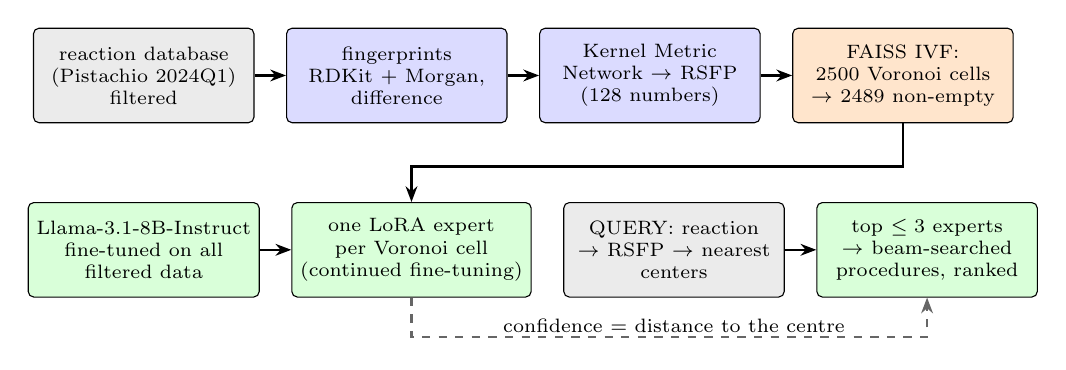
\begin{tikzpicture}[
  box/.style={draw, rounded corners=2pt, minimum height=1.2cm, minimum width=2.8cm, align=center, font=\scriptsize, inner sep=3pt},
  gray/.style={box, fill=black!8},
  bl/.style={box, fill=blue!14},
  og/.style={box, fill=orange!20},
  gr/.style={box, fill=green!15},
  arr/.style={-{Stealth[length=2mm]}, thick}
]
\node[gray] (db) {reaction database\\(Pistachio 2024Q1)\\filtered};
\node[bl, right=0.4cm of db] (fp) {fingerprints\\RDKit + Morgan,\\difference};
\node[bl, right=0.4cm of fp] (kmn) {Kernel Metric\\Network $\to$ RSFP\\(128 numbers)};
\node[og, right=0.4cm of kmn] (vor) {FAISS IVF:\\2500 Voronoi cells\\$\to$ 2489 non-empty};
\draw[arr] (db)--(fp); \draw[arr] (fp)--(kmn); \draw[arr] (kmn)--(vor);
\node[gr, below=1.0cm of db] (base) {Llama-3.1-8B-Instruct\\fine-tuned on all\\filtered data};
\node[gr, right=0.4cm of base] (exp) {one LoRA expert\\per Voronoi cell\\(continued fine-tuning)};
\node[gray, right=0.4cm of exp] (q) {QUERY: reaction\\$\to$ RSFP $\to$ nearest\\centers};
\node[gr, right=0.4cm of q] (out) {top $\le3$ experts\\$\to$ beam-searched\\procedures, ranked};
\draw[arr] (vor.south) -- ++(0,-0.55) -| (exp.north);
\draw[arr] (base)--(exp); \draw[arr] (q)--(out); \draw[arr, dashed, black!60] (exp.south) -- ++(0,-0.5) -| (out.south);
\node[font=\scriptsize, below=0.15cm of q] {confidence $=$ distance to the centre};
\end{tikzpicture}
\caption{MOSAIC. Top row: building the map of reaction space and its Voronoi cells. Bottom row: the experts and their use. Experts are language models fine-tuned on the reactions of one cell; a query is routed to the nearest few cells.}
\label{fig:mosaic}
\end{figure}

Each expert is the Llama-3.1-8B-Instruct language model plus a small \textbf{LoRA adapter}. The authors fine-tune in two stages: first a \textbf{base model} on the whole filtered data set, then each expert \emph{continues} from that base on the reactions of its own cell. The reason, in their words, is that the experts keep the broad knowledge of chemical nomenclature and of the physical state of substances while specializing in their reaction domain. Training thousands of small, independent models is also easy to run in parallel (no synchronization between GPU nodes), compared with training one model on all the data across many devices.

\textbf{LoRA in one line.} Instead of retraining a weight matrix $W$, learn a low-rank update $W'=W+\frac\alpha rBA$ with $B\in\R^{d_{\rm out}\times r}$, $A\in\R^{r\times d_{\rm in}}$, adding only $r(d_{\rm in}+d_{\rm out})$ parameters (Supplement~\hyperref[sec:S4]{S4}). The paper does not state the rank or which layers are adapted (this is in the authors' training scripts, which we did not read), so the sizes below are an \emph{illustration}:

\begin{center}
\small
\begin{tabular}{@{}lcccc@{}}
\toprule
Illustrative adapter & Parameters & Share of the 8.03 B base & Size (16-bit) & 2498 adapters\\
\midrule
rank 8, attention only & $6.8$ M & $0.08\%$ & $14$ MB & $34$ GB\\
rank 16, attention only & $13.6$ M & $0.17\%$ & $27$ MB & $68$ GB\\
rank 16, all linear layers & $41.9$ M & $0.52\%$ & $84$ MB & $210$ GB\\
\bottomrule
\end{tabular}
\end{center}

Whatever the exact configuration, the arithmetic explains the design: $2498$ full copies of the model would need about $40$ TB, whereas a collection of adapters of this size fits on a single disk, and ``loading an expert'' means swapping a few tens of megabytes onto a model that is already in memory.

\tryit{Primer \S10. Derive the parameter count of Llama-3.1-8B and the adapter sizes from the architecture.}

% =============================================================
\section{Step 5: The prompt is a chain of steps}
% =============================================================
The experts are prompted in a fixed format inspired by Stanford Alpaca. Because a language model writes one token after another, the prompt is arranged so that each stage conditions the next (Figure~2a of the preprint):
\begin{enumerate}[nosep]
  \item the \textbf{product and reactant} (SMILES): the transformation;
  \item the \textbf{atom-mapped reaction} with reagents and solvents, still in SMILES;
  \item the \textbf{reagent and solvent} SMILES derived from that mapping;
  \item the same molecules as \textbf{chemical names} or accepted abbreviations;
  \item the \textbf{reaction procedure} in natural language, using these names;
  \item the \textbf{reaction classification} and the \textbf{yield} and characterization.
\end{enumerate}
The structured part comes first, and the free-text procedure only after the model has committed to a mapping and to named reagents. In a comparison on $12$ reactions, atom mapping was the task on which MOSAIC stood out most: the commercial models in the test identified the reaction class but consistently failed to produce the mapping.

% =============================================================
\section{Step 6: Prediction, confidence and what to try first}
% =============================================================
\textbf{Routing.} A query reaction is encoded by the KMN to an RSFP, FAISS finds the nearest Voronoi centers, and the corresponding experts (up to three in the paper's experiments) each write procedures by beam search: in the validation experiments, a beam size of $20$ with $2$ to $20$ beam groups.

\textbf{Confidence is a distance.} The confidence of a prediction is the distance between the query's RSFP and the centroid of the expert that produced it. The authors describe three regimes: distances below $50$ mean a close structural and mechanistic resemblance (high confidence); $100$ to $200$ a recognizable core transformation with different substrates (moderate); above $200$ only the same broad reaction category. Queries at distance $300$ still returned useful analogies, e.g. an aryl iodide coupling for an aryl bromide query. Because FAISS reports \emph{squared} Euclidean distances, these are presumably squared distances ($50$ would be a Euclidean distance of $7.1$ and $200$ of $14.1$; our reading).

\textbf{What the toy shows.} Grouping the $2000$ toy test reactions into quintiles by the squared distance to their nearest center, the one-shot exact match rate for the reagent set is

\begin{center}
\small
\begin{tabular}{@{}lccccc@{}}
\toprule
Distance quintile & closest & 2 & 3 & 4 & farthest\\
\midrule
Exact reagent match (\%) & $48.5$ & $50.2$ & $49.2$ & $36.8$ & $8.8$\\
\bottomrule
\end{tabular}
\end{center}

(Spearman correlation between distance and success $-0.27$.) Two lessons. Distance is a useful \emph{warning}: the farthest fifth of the queries succeeds more than five times less often. But it is not a probability of being right: even the closest queries succeed only half the time, because the true conditions in this toy are genuinely multi-modal. A small distance means ``inside the expert's domain,'' not ``correct.''

\textbf{Which experiment first? (Experiment prioritization.)} With $N$ experts, where expert $e$ offers $M_e$ predictions, the preprint ranks prediction $p$ of expert $e$ by
\[
  R(e,p)=N\,(p-1)+e ,
\]
so that every expert's first prediction is tried before any expert's second. For $N=3$ and $M=(4,2,3)$ the ranks are $1,2,3,4,5,6,7,9,10$: expert $2$ runs out after its second prediction, so the ranks $8$ and $11$ never occur. The ranks order the experiments but are not consecutive.

\tryit{Primer \S6 and \S8. Distance quintiles on the toy; the ranking rule.}

% =============================================================
\section{Step 7: Evaluation}
% =============================================================
\subsection*{Reagents and solvents: a set metric}
The authors compare the predicted set $S_{\rm pred}$ of reagents (or solvents) with the true set $S_{\rm true}$ from the database using
\[
  D=1-\frac{|S_{\rm pred}\cap S_{\rm true}|}{|S_{\rm true}|}.
\]
$D=0$ means that the \textbf{true set is contained in the predicted set} (an ``exact match''); $D<1$ means at least one true molecule appears among the predicted ones (a ``partial match''). In \emph{one-shot} mode only the best beam of the closest expert is used; in \emph{multiple-shots} mode, predictions of up to three experts are aggregated. Results of the preprint (percent of reactions; ``both'' treats reagents and solvents as one set):

\begin{center}
\small
\begin{tabular}{@{}llccc@{}}
\toprule
 & Match & Reagent & Solvent & Both\\
\midrule
One-shot & exact & $22.4$ & $29.8$ & $12.9$\\
 & partial & $45.4$ & $51.7$ & $73.0$\\
Multiple-shots & exact & $43.0$ & $32.8$ & $28.9$\\
 & partial & $76.0$ & $55.2$ & $94.8$\\
\bottomrule
\end{tabular}
\end{center}

\textbf{What the table says} (all derived from the numbers above). The fraction of reactions for which \emph{not one} correct reagent or solvent is predicted drops from $27.0\%$ to $5.2\%$, a factor of $5.2$. Reagents gain a lot from extra experts (exact match $\times1.92$, partial $\times1.67$); solvents gain little ($\times1.10$, $\times1.07$). If the three experts covered the truth independently, each with the one-shot probability $q$, the three-expert rate would be $1-(1-q)^3$. Solving $1-(1-q)^m=\text{observed}$ for $m$ gives the \emph{effective number of independent experts} among the three:

\begin{center}
\small
\begin{tabular}{@{}lcccccc@{}}
\toprule
 & \multicolumn{2}{c}{Reagent} & \multicolumn{2}{c}{Solvent} & \multicolumn{2}{c}{Both}\\
 & exact & partial & exact & partial & exact & partial\\
\midrule
Independence prediction (\%) & $53$ & $84$ & $65$ & $89$ & $34$ & $98$\\
Observed (\%) & $43$ & $76$ & $33$ & $55$ & $29$ & $95$\\
Effective independent experts & $2.2$ & $2.4$ & $1.1$ & $1.1$ & $2.5$ & $2.3$\\
\bottomrule
\end{tabular}
\end{center}

The three nearest experts behave like about two and a quarter independent experts for reagents, and like barely one for solvents, which means they nearly always suggest the same solvent. This is consistent with the idea that experts of neighboring cells have overlapping knowledge, and it is a crude model (it assumes equal coverage probability), but it shows where extra experts help.

\subsection*{A critical look at ``exact match''}
Because $D=0$ whenever the true set is \emph{contained} in the prediction, a prediction that lists more molecules can only do better. Pooling the predictions of several experts enlarges the predicted set, so part of the improvement from one-shot to multiple-shots is mechanical, and the metric as defined does not penalize it. The extreme case is to predict \emph{every} reagent: it is an exact match $100\%$ of the time. The toy makes the trade-off visible, pooling more experts in the toy universe:

\begin{figure}[ht]
\centering
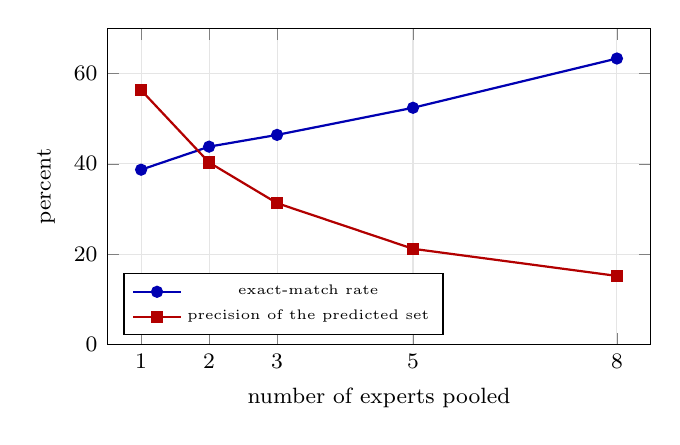
\begin{tikzpicture}
\begin{axis}[width=0.7\textwidth, height=5.6cm, xlabel={number of experts pooled}, ylabel={percent}, xmin=0.5, xmax=8.5, ymin=0, ymax=70, xtick={1,2,3,5,8},
  grid=major, grid style={black!10}, legend pos=south west, legend style={font=\tiny}, tick label style={font=\footnotesize}, label style={font=\footnotesize}]
\addplot[blue!70!black, thick, mark=*, mark size=1.8pt] coordinates {(1,38.7) (2,43.8) (3,46.4) (5,52.4) (8,63.3)};
\addplot[red!70!black, thick, mark=square*, mark size=1.8pt] coordinates {(1,56.3) (2,40.3) (3,31.3) (5,21.2) (8,15.2)};
\legend{exact-match rate, precision of the predicted set}
\end{axis}
\end{tikzpicture}
\caption{Toy universe, reagent prediction. Each added expert raises the exact-match rate (blue) from $38.7\%$ to $63.3\%$, but the predicted set grows from $2.0$ to $11.2$ molecules and its precision (the share of predicted molecules that are correct) falls from $56.3\%$ to $15.2\%$. Predicting all $30$ reagents scores $100\%$ exact match and $7.0\%$ precision.}
\label{fig:prec}
\end{figure}

This does not mean that MOSAIC's results are inflated: the preprint's drop of the ``nothing right'' rate from $27.0\%$ to $5.2\%$ is a genuine gain in coverage, and the paper reports the \emph{one-shot} numbers as well. It means that Table~1 should be read together with the \emph{size} of the predicted sets (or the precision), which the preprint does not give in the main text. For a chemist, the quantity that matters is how many experiments she must run to hit a working condition, which is what the ranking rule above is for.

\subsection*{Yield prediction}
The model writes the yield as text, not as a number from a regression head. To evaluate it, the preprint groups yields into ten bins of $10$ percentage points, and plots the median predicted yield of each bin against the average true yield of its members. Its figure has two panels (reaction classes capped at $20$ examples, and unconstrained), with fit lines labelled $y=0.61x+24.99$ and $y=0.61x+24.93$.

\begin{figure}[ht]
\centering
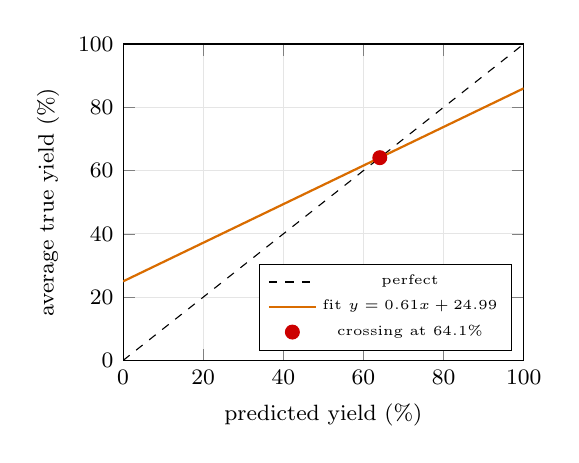
\begin{tikzpicture}
\begin{axis}[width=0.55\textwidth, height=5.6cm, xlabel={predicted yield (\%)}, ylabel={average true yield (\%)}, xmin=0, xmax=100, ymin=0, ymax=100, grid=major, grid style={black!10},
  legend pos=south east, legend style={font=\tiny}, tick label style={font=\footnotesize}, label style={font=\footnotesize}]
\addplot[black, dashed] coordinates {(0,0) (100,100)};
\addplot[orange!85!black, thick] coordinates {(0,24.99) (100,85.99)};
\addplot[only marks, mark=*, mark size=2.5pt, red!80!black] coordinates {(64.08,64.08)};
\legend{perfect, fit $y=0.61x+24.99$, crossing at $64.1\%$}
\end{axis}
\end{tikzpicture}
\caption{The fit of the preprint's yield figure. A slope of $0.61$ means the predictions are informative but over-dispersed.}
\label{fig:yield}
\end{figure}

Taking the fit at face value (derived): the line crosses $y=x$ at $b/(1-a)=24.99/0.39=64.1\%$; a predicted yield of $5\%$ corresponds to an average true yield of $28\%$ and a predicted $95\%$ to $82.9\%$. The slope of $0.61$ below $1$ is the familiar \emph{regression to the mean}: a spread of $90$ points in predictions goes with $55$ points in truth. A linear recalibration $x\mapsto(y-24.99)/0.61$ would undo the compression but not the scatter within each bin, which the preprint shows only in a figure. The authors describe this as a ``qualitative understanding of yield trends,'' and note that bespoke yield models trained on curated data sets are more precise for their narrow tasks, while MOSAIC covers a far broader range.

\subsection*{Comparison with general-purpose language models}
On $12$ reactions of six types (Suzuki, olefin metathesis, Buchwald--Hartwig, Heck, Sonogashira, esterification) on novel substrates, MOSAIC was scored against GPT-4o mini, Claude 3.5 Haiku, Claude 3.5 Sonnet and ChatGPT-o1 Pro with a rubric: atom mapping ($1$ point), reagents and solvents ($1$--$2$), experimental operations ($1$), quantitative parameters ($1$--$2$), workup ($1$), classification ($1$), and a $-2$ penalty for ignoring instructions; each prompt was repeated three times. Responses scoring below $5.0$ were judged unusable in practice. The preprint reports MOSAIC ahead in all categories. Two caveats: the models in this comparison date from late 2024, and the rubric is applied by the authors; the comparison is a snapshot of that time, not a statement about today's models.

\tryit{Primer \S4--5 and \S7. Score the toy specialists with the set metric, measure precision, and recompute the effective number of independent experts from Table~1.}

% =============================================================
\section{Step 8: Experimental validation}
% =============================================================
The strongest part of the paper is that the predictions were carried out at the bench. Up to three experts were used per compound; the highest-ranked predictions were tried first, and for novel transformation types where confidence was low, additional predictions were tested. The preprint reports more than $35$ new compounds, across:
\begin{itemize}[nosep]
  \item \textbf{Cross-couplings:} Suzuki (biaryl fragments containing sensitive functional groups), Heck (including a case where a literature attempt had failed), Buchwald--Hartwig and Goldberg aminations (derivatives of nortriptyline and fenofibrate), Sonogashira (a dual-catalyst system), diaryl ether synthesis (estrone derivatives), and olefin metathesis (late-stage modification of an adhesive component and a ring-opening metathesis monomer).
  \item \textbf{Selectivity-demanding transformations:} a chromium-free controlled oxidation to an aldehyde, conjugate addition to (S)-carvone, prenylation of sclareolide, a Horner--Wadsworth--Emmons olefination of L-perillaldehyde, and selective silyl protection of hesperetin.
  \item \textbf{Applications:} new drug-like molecules and modifications of existing drugs (labelled celecoxib, donepezil and amoxapine in the figure), a bipyridine ligand and photocatalyst analogues, conjugated materials, pyrabactin analogues for agrochemistry, hedione-derived fragrance analogues and citronellyl retinoate for cosmetics, and a new heterocycle synthesis.
\end{itemize}
Summing up the yields printed in the preprint's Figures~3 and~4 ($37$ entries; derived): they range from $19\%$ to $96\%$, with a median of $71\%$ and quartiles of $45\%$ and $83\%$; two entries are NMR yields. Most entries list a single trial, a few two or four.

\textbf{How to read that.} These are \emph{successful} syntheses selected for the figures: the main text we read does not state how many compounds were attempted, or how many first-ranked predictions failed (the preprint refers to a supplementary section for all trials). So the figures show that the approach \emph{can} produce working procedures for new compounds, which is what a demonstration needs, but they do not give a success rate. The authors' own discussion lists a failure mode too: for symmetric multiple functionalization, no valid predictions were produced from the top two experts.

% =============================================================
\section{Step 9: Reading the evidence critically}
% =============================================================
\sloppy
\begin{enumerate}[nosep]
  \item \textbf{The limitations the authors state.} MOSAIC adapts known reaction patterns and \emph{cannot discover entirely new transformations} involving unprecedented reagents. It trades some precision for breadth. It inherits the tokenization limits of language models, which struggle to translate between SMILES and names for large, multi-heterocyclic molecules, although functional groups and reaction patterns are still recognized.
  \item \textbf{The data are proprietary.} Training from scratch needs the commercial Pistachio database (the repository's README says to ``set up the Pistachio database, or use any custom databases'' and contains a file named \texttt{Pistachio\_Sample\_100.csv}, which we did not open); results cannot be reproduced without a license.
  \item \textbf{Match rates and set sizes.} As in Step~7, the exact-match rates of the preprint must be read together with the size of the predicted sets.
  \item \textbf{Confidence is relative.} The distance thresholds are descriptive; they are not calibrated probabilities. The toy shows how a calibration could be done on held-out data: bin by distance, and report the observed success rate of each bin.
  \item \textbf{Successes are shown, attempts are not.} See Step~8.
  \item \textbf{A snapshot in time.} The comparison with commercial models used the models of late 2024, and the numbers here are from the preprint, not the published version.
  \item \textbf{Safety.} The authors state that all procedures generated by MOSAIC must only be carried out by trained individuals in properly equipped laboratories, since procedures may omit hazards. Procedures written by a language model are suggestions, not a substitute for a hazard assessment.
\end{enumerate}

% =============================================================
\section{Run it yourself}
\label{sec:runit}
% =============================================================
\begin{keybox}[Which notebook?]
\begin{description}[leftmargin=0pt, nosep, labelindent=0pt]
  \item[Primer] \colabbutton{\colaburlprimer}{Open the primer}\ \ \texttt{B6c\_mosaic\_primer\_colab.ipynb}. CPU only, about ten seconds, NumPy, SciPy, pandas. It runs a synthetic reaction universe through every mechanism described above and ends with a self-check cell. It runs no language model. Start here.
  \item[The authors' repository] \colabbutton{\urlrepo}{Open the repository}\ \ \texttt{batistagroup/MOSAIC}, ``the official implementation'' of the \emph{Nature} paper (a fork of \texttt{haoteli/MOSAIC}). Its README lists the requirements (Python $\ge3.11.9$; PyTorch $2.4.1$, RDKit $2023.9.6$, FAISS $1.7.4$, Transformers $4.45.1$, PEFT $0.12.0$, TRL $0.11.1$, among others) and the structure: \texttt{DataProcessing} (fingerprints; Voronoi domains), \texttt{KernelMetricNetwork}, \texttt{Training} (first fine-tuning; expert fine-tuning), \texttt{PredictionUtils}, \texttt{Main\_Control.ipynb} (examples), \texttt{MOSAIC\_Add\_Expert\_Demo.ipynb} and a \texttt{Model\_Weights} folder, plus a license file. We have \emph{not} run any of it, did not inspect the weights folder, and did not read the license; you need GPUs, the Llama weights (under Meta's license) and the Pistachio data to train. The authors also host a web playground for their models at \url{https://models.batistalab.com} (which we did not use).
\end{description}
\end{keybox}

\subsection{Where each step lives in the primer}
\begin{center}
\small
\begin{tabular}{@{}llp{6.5cm}@{}}
\toprule
Post & Primer & What you should see\\
\midrule
Step 2 & \S1--2 & 1-NN accuracy $0.825$ raw, $0.978$ difference, $0.997$ RSFP\\
Step 3 & \S3 & $30$ cells; IVF recall $0.943$ at $5.0\%$ scanned ($1$ probe)\\
Steps 6--7 & \S4--6 & toy exact/partial rates; precision falls as experts are pooled; distance quintiles\\
Step 7 & \S7, \S9 & $27.0\%\to5.2\%$; effective experts $2.2$ vs $1.1$; fit crosses at $64.1\%$\\
Step 6 & \S8 & ranks $1,2,3,4,5,6,7,9,10$\\
Step 4 & \S10 & $8.03$ B parameters; adapters $14$--$84$ MB; $40$ TB vs $210$ GB\\
\bottomrule
\end{tabular}
\end{center}

\subsection{The key calculations in one cell}
This script needs only the Python standard library:

\begin{lstlisting}
# 1) the paper's set metric: D = 0 means the TRUE set is contained in the PREDICTED set
D = lambda pred, true: 1 - len(pred & true) / len(true)
print("D({A,B} vs {A,C,D}) =", D({"A", "C", "D"}, {"A", "B"}), "| D({A,B} vs {A,B,C,D,E}) =", D({"A", "B", "C", "D", "E"}, {"A", "B"}))

# 2) the experiment-ranking rule R(e, p) = N (p - 1) + e, for experts offering M = [4, 2, 3] predictions
M = [4, 2, 3]; N = len(M)
print("ranks:", sorted(N * (p - 1) + e for e in range(1, N + 1) for p in range(1, M[e - 1] + 1)))

# 3) what the preprint's Table 1 implies (percent of reactions)
partial_both = {"one-shot": 73.0, "multiple-shots": 94.8}
fail = {k: 100 - v for k, v in partial_both.items()}
print(f"no correct reagent or solvent predicted: {fail['one-shot']:.1f} % -> {fail['multiple-shots']:.1f} % ({fail['one-shot'] / fail['multiple-shots']:.1f}x fewer)")
print(f"reagent exact match, multiple-shots / one-shot: {43.0 / 22.4:.2f}; solvent: {32.8 / 29.8:.2f}")

# 4) the preprint's yield fit y = 0.61 x + 24.99
print(f"fit crosses y = x at {24.99 / (1 - 0.61):.1f} % yield; a predicted 95 % corresponds to {0.61 * 95 + 24.99:.1f} % true on average")

# 5) Llama-3.1-8B and an illustrative LoRA adapter (the real rank and target layers are not in the paper)
h, layers, inter, heads, kv_heads, vocab = 4096, 32, 14336, 32, 8, 128_256
kv = kv_heads * (h // heads)
attn = 2 * h * h + 2 * h * kv; mlp = 3 * h * inter
base = 2 * vocab * h + layers * (attn + mlp + 2 * h) + h
lora = lambda r: layers * r * (6 * h + 2 * kv + 3 * (h + inter))          # q, k, v, o, gate, up, down
print(f"base model {base / 1e9:.2f} B parameters; LoRA rank 16 on all linear layers: {lora(16) / 1e6:.1f} M parameters = {100 * lora(16) / base:.2f} % of the base")
print(f"2498 adapters: {2498 * 2 * lora(16) / 1e9:.0f} GB; 2498 full 16-bit copies: {2498 * 2 * base / 1e12:.0f} TB")
\end{lstlisting}

Expected output:
\begin{lstlisting}[language={},basicstyle=\ttfamily\small]
D({A,B} vs {A,C,D}) = 0.5 | D({A,B} vs {A,B,C,D,E}) = 0.0
ranks: [1, 2, 3, 4, 5, 6, 7, 9, 10]
no correct reagent or solvent predicted: 27.0 % -> 5.2 % (5.2x fewer)
reagent exact match, multiple-shots / one-shot: 1.92; solvent: 1.10
fit crosses y = x at 64.1 % yield; a predicted 95 % corresponds to 82.9 % true on average
base model 8.03 B parameters; LoRA rank 16 on all linear layers: 41.9 M parameters = 0.52 % of the base
2498 adapters: 210 GB; 2498 full 16-bit copies: 40 TB
\end{lstlisting}

\subsection{Experiments worth five minutes}
\begin{itemize}[nosep]
  \item \textbf{More or fewer cells.} Change \texttt{K} from $30$ to $10$ and to $100$ in the primer. How do the class purity and the IVF recall change?
  \item \textbf{Precision matters.} Define an F1-style score from the exact-match rate and the precision. At how many pooled experts is it highest?
  \item \textbf{A calibration.} Turn the distance quintiles into a table of observed success rates, and decide at which distance you would stop trusting the nearest expert.
  \item \textbf{Bigger adapters.} Compute the size of one adapter and the whole collection for rank $64$ on all linear layers ($168$ M parameters, $336$ MB, $0.84$ TB).
\end{itemize}

% =============================================================
\section{What to take away}
% =============================================================
\begin{keybox}[Summary]
\begin{itemize}[nosep]
  \item \textbf{Many small specialists, one map.} MOSAIC does not use one huge model. It learns a map of reaction space (fingerprints $\to$ a $128$-dimensional learned similarity), cuts it into about $2500$ Voronoi cells with FAISS, and trains one LoRA-adapted Llama-3.1-8B expert per cell.
  \item \textbf{A learned metric beats raw fingerprints.} In the toy, nearest-neighbor class accuracy goes from $0.83$ (raw) to $0.997$ (learned); the real system trains its metric to classify $2285$ reaction classes.
  \item \textbf{Confidence is a distance.} The distance from the query to the expert's centroid is a cheap, interpretable warning (the farthest quintile succeeds more than five times less often in the toy), but it is not a calibrated probability.
  \item \textbf{More experts, fewer total misses.} In the preprint, using up to three experts lowers the share of reactions with not one correct reagent or solvent from $27.0\%$ to $5.2\%$; the three experts behave like $2.2$ independent experts for reagents and $1.1$ for solvents.
  \item \textbf{Read ``exact match'' with set sizes.} The metric counts a prediction as exact if it \emph{contains} the truth, so pooling experts raises it mechanically; precision falls.
  \item \textbf{Scale arithmetic explains the design.} Adapters are tens of megabytes and the collection fits on a disk ($\sim$\,$200$ GB for an illustrative rank $16$), against $\sim$\,$40$ TB for full copies; IVF search scans a few thousand vectors instead of a million.
  \item \textbf{What is shown, and not.} More than $35$ new compounds were made, with a median listed yield of about $70\%$; the number of attempts is not in the main text. MOSAIC adapts known patterns and cannot invent new reagents.
\end{itemize}
\end{keybox}

\textbf{Next in the series (B7):} predicting dynamics with dynamic mode decomposition.

\vspace{0.5em}
{\footnotesize\textbf{Credits.} MOSAIC is by H.~Li, S.~Sarkar, W.~Lu, P.~O.~Loftus, T.~Qiu, Y.~Shee, A.~E.~Cuomo, J.-P.~Webster, H.~R.~Kelly, V.~Manee, S.~Sreekumar, F.~G.~Buono, R.~H.~Crabtree, T.~R.~Newhouse and V.~S.~Batista (Yale University and Boehringer Ingelheim), \emph{Nature} \textbf{651}, 107--115 (2026), DOI 10.1038/s41586-026-10131-4; preprint \emph{Collective intelligence of specialized language models guides realization of de novo chemical synthesis}, ChemRxiv 10.26434/chemrxiv-2025-dc28b (license CC BY-NC-ND 4.0); code at \url{https://github.com/batistagroup/MOSAIC} (official implementation; forked from \texttt{haoteli/MOSAIC}). The primer notebook is an independent toy implementation of the mechanisms described and contains none of the authors' code or data.}

\clearpage
% =============================================================
\section*{Supplementary Reading: The Math}
\addcontentsline{toc}{section}{Supplementary Reading: The Math}
% =============================================================
\textit{Prerequisites: vectors and Euclidean distance (Toolbox T2), probability (T3), and Post B6 (transformers) for the autoregressive factorization.}

\phantomsection\label{sec:S1}
\subsection*{S1. Reaction fingerprints and the difference fingerprint}
A molecule fingerprint is a bit vector $x\in\{0,1\}^n$ whose bit $j$ records whether substructure $j$ is present (hashed, so different substructures may collide). For a reaction with reactant fingerprint $r$ and product fingerprint $p$ the difference fingerprint is
\[
  d=p-r\in\{-1,0,+1\}^n,\qquad d_j=\begin{cases}+1&\text{substructure created},\\-1&\text{substructure destroyed},\\0&\text{unchanged}.\end{cases}
\]
Substructures that merely sit elsewhere in the molecule appear in both $r$ and $p$ and cancel in $d$; what remains is the transformation. MOSAIC concatenates $[r,\,p,\,d]$ (with two kinds of fingerprints, RDKit and Morgan). In the toy of the primer, the substrate contributes random bits to $r$ and $p$ (large distances between reactions of the same class), while $d$ contains only the class pattern, which is why the difference alone already gives a $1$-NN accuracy of $0.978$ against $0.825$ for $[r,p,d]$.

\phantomsection\label{sec:S2}
\subsection*{S2. Metric learning by classification}
Let $\phi:\R^{n}\to\R^{128}$ be the network up to the RSFP layer and $W\in\R^{128\times C}$, $b\in\R^C$ the output layer, with $C$ classes ($C=2285$ in the paper). Training minimizes the cross-entropy $-\ln\softmax(\phi(x)^{\!\top}W+b)_y$. After training, points of one class have logits dominated by the same column of $W$, so $\phi(x)$ lies in a cone around $W_{\cdot y}$; the layer's geometry therefore puts same-class points close and, for related classes with similar columns, nearby. The distance
\[
  \lVert\phi(x)-\phi(x')\rVert^2=\sum_{i=1}^{128}\big(\phi_i(x)-\phi_i(x')\big)^2
\]
is the quantity of Eq.~1 of the preprint. Nothing forces classification training to produce a good metric (the loss never compares two points directly), which is why the quality of the space is checked, as in the toy: $1$-NN accuracy in the learned space ($0.997$) against raw ($0.825$).

\phantomsection\label{sec:S3}
\subsection*{S3. Voronoi cells, $k$-means and the cost of IVF search}
Given centroids $c_1,\dots,c_K$, the \textbf{Voronoi cell} of $c_k$ is $V_k=\{z:\lVert z-c_k\rVert^2\le\lVert z-c_j\rVert^2\ \forall j\}$. Lloyd's algorithm for $k$-means alternates assigning each point to its nearest centroid and replacing each centroid by the mean of its points; it decreases $\sum_i\lVert z_i-c_{a(i)}\rVert^2$ at every step and stops at a local minimum. IVF uses these cells as an inverted index.

\paragraph{Cost.} For $N$ vectors in $K$ cells of equal size and a search of the \texttt{nprobe} nearest cells,
\[
  \text{cost}(K)\approx K+\texttt{nprobe}\cdot\frac NK,\qquad K^\ast=\sqrt{\texttt{nprobe}\cdot N}.
\]
For $N=10^6$: $K^\ast=1000$ ($\texttt{nprobe}=1$) or $1732$ ($\texttt{nprobe}=3$), with cost $2000$ or $3464$. With the paper's $K=2500$ the cost is $2900$ or $3700$, close to the minimum. In MOSAIC, the number of cells is also the number of experts, so it is set by how much data each expert should see ($\sim400$ reactions) and not only by the search cost.

\paragraph{Recall.} IVF is approximate: if the true nearest neighbor lies in a cell that is not probed, it is missed. In the toy, recall is $0.943,0.993,0.999,1.000$ for $\texttt{nprobe}=1,2,3,5$ while scanning $5.0,9.3,13.1,21.4\%$ of the data.

\phantomsection\label{sec:S4}
\subsection*{S4. LoRA and the arithmetic of 2498 experts}
For a frozen weight matrix $W\in\R^{d_{\rm out}\times d_{\rm in}}$, LoRA trains $B\in\R^{d_{\rm out}\times r}$ and $A\in\R^{r\times d_{\rm in}}$ and uses $W'=W+\frac\alpha rBA$, usually with $B=0$ at initialization so that training starts exactly from the base model. The adapter has $r(d_{\rm in}+d_{\rm out})$ parameters against $d_{\rm in}d_{\rm out}$ for the matrix.

\paragraph{Llama-3.1-8B.} Hidden size $h=4096$, $32$ layers, $32$ attention heads with $8$ key-value heads (so the key and value projections map $4096\to1024$), feed-forward size $14{,}336$, vocabulary $128{,}256$. Per layer: attention $2h^2+2h\cdot1024=41.9$ M; feed-forward $3h\cdot14{,}336=176.2$ M. In total $2\cdot128{,}256\cdot4096$ for the embedding and output layers, plus $32\times(41.9+176.2)$ M for the blocks, plus small norms: $8.03$ billion parameters, $16.1$ GB in $16$-bit.

\paragraph{Adapters.} Rank $16$ on all seven linear layers of a block gives, per block, $16\,[\,(h+h)+(h+1024)+(h+1024)+(h+h)+3(h+14336)\,]=1.31$ M, so $41.9$ M for $32$ blocks, $0.52\%$ of the base. With rank $8$ on the four attention projections: $6.8$ M. The paper does not give the actual rank or targets; these are illustrations. A collection of $2498$ adapters of $84$ MB is $210$ GB; the same number of full copies is $2498\times16.1$ GB $=40$ TB.

\paragraph{Training cost.} The experts are trained on disjoint parts of the data, so one epoch over all of them processes about as many examples as one epoch over the whole data set, plus the base fine-tuning: roughly twice the cost of a single pass (derived), but with no communication between the jobs.

\phantomsection\label{sec:S5}
\subsection*{S5. The staged prompt and beam search}
A decoder-only language model writes a sequence $y=(y_1,\dots,y_T)$ with probability $p(y\mid x)=\prod_tp(y_t\mid x,y_{<t})$. MOSAIC's prompt arranges the content as $s=1,\dots,6$ stages (transformation, atom-mapped reaction, reagents and solvents as SMILES, names, procedure, classification and yield), each generated conditioned on the previous ones, so that the free-text procedure is conditioned on the structured, checkable content. \textbf{Beam search} keeps the $B$ highest-scoring partial sequences, scored by $\sum_t\ln p(y_t\mid x,y_{<t})$; with $B=20$ it returns up to $20$ candidate procedures per expert, and \emph{diverse} beam search (beam groups) penalizes groups for repeating one another's tokens, which makes the candidates differ.

For yield, the model emits a token string for the number. The preprint obtains a numeric prediction by averaging across the beam-searched results (its Fig.~2c), so a yield prediction is the average of several candidate completions.

\phantomsection\label{sec:S6}
\subsection*{S6. The set metric, and what pooling experts does to it}
With $S_{\rm pred}$ and $S_{\rm true}$ sets of molecules, define recall $\rho=|S_{\rm pred}\cap S_{\rm true}|/|S_{\rm true}|$ and precision $\pi=|S_{\rm pred}\cap S_{\rm true}|/|S_{\rm pred}|$. The paper's metric is $D=1-\rho$. An \textbf{exact match} is $\rho=1$, i.e.\ $S_{\rm true}\subseteq S_{\rm pred}$; a \textbf{partial match} is $\rho>0$. Neither involves $\pi$.

\paragraph{Pooling is monotone.} If $S_{\rm pred}^{(n)}=\bigcup_{k\le n}S_k$ is the union of the predictions of the $n$ nearest experts, then $S_{\rm pred}^{(n)}\subseteq S_{\rm pred}^{(n+1)}$, so $\rho$ cannot decrease and the exact- and partial-match rates are non-decreasing in $n$; at the same time $|S_{\rm pred}^{(n)}|$ is non-decreasing and $\pi$ typically falls. The extreme $S_{\rm pred}=$ all molecules has $\rho=1$ and $\pi=|S_{\rm true}|/|\text{all}|$.

\paragraph{Effective number of independent experts.} Suppose each of $n$ experts covers the true set independently with the same probability $q$. Then the pooled coverage is $1-(1-q)^n$. Given the observed pooled rate $f$ at $n=3$ and the one-shot rate $q$, the effective number $m$ solves $1-(1-q)^m=f$, i.e.
\[
  m=\frac{\ln(1-f)}{\ln(1-q)}.
\]
For reagent exact match, $q=0.224$, $f=0.430$: $m=\ln0.570/\ln0.776=2.22$. For solvent exact match, $q=0.298$, $f=0.328$: $m=\ln0.672/\ln0.702=1.12$. Positive correlation between experts' successes makes $m<n$; $m\approx1$ means the experts are interchangeable. Under independence the predicted pooled rates would be $53\%$ (reagent) and $65\%$ (solvent), against the observed $43\%$ and $33\%$.

\paragraph{Table 1 sanity checks.} Partial $\ge$ exact in every column; the ``both'' partial rate ($73.0\%$ and $94.8\%$) is at least the larger of the reagent and solvent partial rates, since finding one correct component in either set counts; and $94.8\%$ is the paper's ``at least some correct component'' rate.

\phantomsection\label{sec:S7}
\subsection*{S7. The ranking rule}
For $N$ experts and expert $e$ with $M_e$ predictions, $R(e,p)=N(p-1)+e$ for $1\le e\le N$, $1\le p\le M_e$. \textbf{Injective:} $R$ determines $p-1=\lfloor(R-1)/N\rfloor$ and $e=R-N(p-1)$. \textbf{Lexicographic:} $R(e,p)<R(e',p')$ iff $p<p'$, or $p=p'$ and $e<e'$. So all first predictions come first (ranks $1..N$), then all second predictions, and so on. \textbf{Gaps:} when expert $e$ has no prediction $p$ the rank $N(p-1)+e$ is skipped, so the ranks are dense only if all $M_e$ are equal. The total number of experiments is $\sum_eM_e$ and the largest rank is at most $N(\max_eM_e-1)+N$. For $N=3$, $M=(4,2,3)$: ranks $1,2,3,4,5,6,7,9,10$, total $9$.

\phantomsection\label{sec:S8}
\subsection*{S8. Yield bins and the regression to the mean}
Predictions are binned into ten intervals of $10$ points; for each bin the median predicted yield $x_b$ and the mean true yield $\bar y_b$ are computed, and a line is fit through the ten points. A fit $\bar y=ax+b$ with $a<1$ means that bins with high predictions have, on average, true yields that are less extreme: if the true yield $Y$ and the prediction $X$ have means $\mu$ and spreads $\sigma_Y,\sigma_X$, the least-squares slope of $Y$ on $X$ is $a=\rho_{XY}\sigma_Y/\sigma_X$, which is below $1$ whenever the correlation is imperfect (or the predictions are more dispersed than the truth). The fixed point of the line, where $x=ax+b$, is $x^\ast=b/(1-a)$: here $24.99/0.39=64.1\%$. Two cautions: the fit is through \emph{binned} quantities, which usually shows a stronger relationship than the unbinned data would, and mixes a median (predictions) with a mean (true yields).

\phantomsection\label{sec:S9}
\subsection*{S9. Distance as confidence}
The confidence of a prediction is $d(z_q,c_k)$, with $z_q$ the RSFP of the query and $c_k$ the centroid of the answering expert. If $d$ is the squared distance (the default of FAISS), thresholds $50,100,200,300$ correspond to Euclidean distances $7.1,10,14.1,17.3$. A cell is a region of the learned space on which the expert was trained: a query far from the centroid is, in the learned metric, unlike most of the training reactions of that expert, so its prediction is an extrapolation. This is a form of \emph{out-of-distribution score}. It is not a probability: the same distance can correspond to different success rates in different regions, since the multi-modality of conditions (toy: $0.55/0.30/0.15$) caps the success rate even at distance zero. To turn a distance into a probability one fits, on held-out reactions, the observed success rate as a function of distance (for example with isotonic regression). In the toy the five distance quintiles have success rates $48.5,50.2,49.2,36.8,8.8\%$.

\subsection*{Check yourself}
\begin{enumerate}
  \item \textbf{The metric.} Compute $D$ for a true set $\{A,B\}$ and predictions $\{A,C,D\}$ and $\{A,B,C,D,E\}$. Which is an exact match? Which is more useful to a chemist?
  \item \textbf{Cells.} Show that a point on the segment between two centroids lies in the cell of the closer one. How does the cell of a centroid change if you move a neighboring centroid away?
  \item \textbf{IVF.} For $N=10^6$ and $K=2500$ cells, how many distance computations does a search with $\texttt{nprobe}=3$ need? For which $K$ is it minimal?
  \item \textbf{LoRA.} Derive the number of parameters of a rank-$r$ adapter on a $4096\times1024$ matrix. Why does $B=0$ at initialization make training start from the base model?
  \item \textbf{Effective experts.} Compute $m$ for the \emph{partial} reagent match ($q=0.454$, $f=0.760$) and for the ``both'' exact match ($q=0.129$, $f=0.289$).
  \item \textbf{Ranking.} For $N=4$ and $M=(3,3,1,2)$, list the first eight experiments in order. Which ranks never occur?
  \item \textbf{Yield.} With $y=0.61x+24.99$, at which predicted yield are prediction and truth equal? A user is told ``predicted yield $20\%$'': what true yield do you expect on average, and why is the unbinned uncertainty larger than the fit suggests?
  \item \textbf{Confidence.} Design an experiment on held-out reactions to turn the distance into a probability of success. What would you plot, and what would make you distrust the result?
\end{enumerate}

\subsection*{References}
{\small\sloppy
\begin{itemize}[nosep, leftmargin=1.2em]
  \item H.~Li, S.~Sarkar, W.~Lu, \emph{et al.}, \textit{Collective intelligence for AI-assisted chemical synthesis}, Nature \textbf{651}, 107--115 (2026).
  \item H.~Li, S.~Sarkar, W.~Lu, \emph{et al.}, \textit{Collective intelligence of specialized language models guides realization of de novo chemical synthesis}, ChemRxiv (2025), doi:10.26434/chemrxiv-2025-dc28b.
  \item A.~Dubey \emph{et al.}, \textit{The Llama 3 herd of models}, arXiv:2407.21783 (2024).
  \item E.~J.~Hu \emph{et al.}, \textit{LoRA: low-rank adaptation of large language models}, arXiv:2106.09685 (2021).
  \item M.~Douze \emph{et al.}, \textit{The Faiss library}, arXiv:2401.08281 (2024); J.~Zobel, A.~Moffat, \textit{Inverted files for text search engines}, ACM Comput.\ Surv.\ \textbf{38}, 6 (2006).
  \item S.~P.~Lloyd, \textit{Least squares quantization in PCM}, IEEE Trans.\ Inf.\ Theory \textbf{28}, 129--137 (1982).
  \item NextMove Software, \textit{Pistachio} (2024), \url{https://www.nextmovesoftware.com/pistachio}.
  \item R.~Taori \emph{et al.}, \textit{Stanford Alpaca: an instruction-following LLaMA model} (2023).
  \item A.~Vaswani \emph{et al.}, \textit{Attention is all you need}, NeurIPS (2017).
  \item A.~C.~Vaucher \emph{et al.}, \textit{Inferring experimental procedures from text-based representations of chemical reactions}, Nat.\ Commun.\ \textbf{12}, 2573 (2021).
  \item H.~Gao \emph{et al.}, \textit{Using machine learning to predict suitable conditions for organic reactions}, ACS Cent.\ Sci.\ \textbf{4}, 1465 (2018).
  \item M.~Andronov \emph{et al.}, \textit{Reagent prediction with a molecular transformer improves reaction data quality}, Chem.\ Sci.\ \textbf{14}, 3235 (2023).
  \item D.~A.~Boiko \emph{et al.}, \textit{Autonomous chemical research with large language models}, Nature \textbf{624}, 570 (2023); A.~M.~Bran \emph{et al.}, \textit{Augmenting large language models with chemistry tools}, Nat.\ Mach.\ Intell.\ (2024).
  \item K.~M.~Jablonka \emph{et al.}, \textit{Leveraging large language models for predictive chemistry}, Nat.\ Mach.\ Intell.\ \textbf{6}, 161 (2024).
  \item D.~Probst, J.-L.~Reymond, \textit{Visualization of very large high-dimensional data sets as minimum spanning trees}, J.\ Cheminform.\ \textbf{12}, 12 (2020). (The tree map.)
\end{itemize}}

\end{document}
